                \documentclass{article}

% Language setting
% Replace `english' with e.g. `spanish' to change the document language
\usepackage[english]{babel}
\usepackage{listings}
\usepackage{xcolor}
\usepackage{float} % Add this line

\usepackage{amsmath}
\usepackage{tikz}

% Remove indentation
\setlength{\parindent}{0pt}

% Add space between paragraphs
\setlength{\parskip}{1em} % Adjust the length as needed


\lstset{
  basicstyle=\ttfamily,
  breaklines=true,
  columns=fullflexible,
  frame=single,
  backgroundcolor=\color{gray!10},
  xleftmargin=15pt,
  xrightmargin=15pt
}

% Set page size and margins
% Replace `letterpaper' with`a4paper' for UK/EU standard size
\usepackage[letterpaper,top=2cm,bottom=2cm,left=3cm,right=3cm,marginparwidth=1.75cm]{geometry}

% Useful packages
\usepackage{amsmath}
\usepackage{graphicx}
\usepackage[colorlinks=true, allcolors=blue]{hyperref}

\title{The BitFusion Bridge Framework}
\author{Bitfinity Team}

\begin{document}
\maketitle

\begin{abstract}
\noindent BitFusion is a Layer-2 builder for Bitcoin:  an open-source framework designed to enable the creation of decentralized bridges between EVM networks and Bitcoin, Bitcoin Runes, and other EVM networks. By leveraging Chain-Key cryptography and a network of on-chain Bitcoin nodes, BitFusion ensures secure bridging of assets from the Bitcoin ecosystem to EVM chains. This framework includes a bridging widget for seamless integration into downstream applications, providing users with a near-native experience. The technology behind BitFusion offers robust, decentralized security for bridging assets across blockchain networks, setting a new standard for decentralised bridging.


\end{abstract}

\tableofcontents

\section{BitFusion Background Assumptions} 
\subsection{Introduction} 

The BitFusion framework serves as foundational infrastructure for Bitcoin Layer-2 solutions. It incorporates a threshold Elliptic Curve Digital Signature Algorithm (tECDSA) for transaction signing, interfaces directly with a network of Bitcoin nodes, and provides bridging capabilities for a diverse array of assets from the Bitcoin ecosystem, including Runes and BTC.

BitFusion leverages committee-based security assumptions, which, despite being an addition to those of the base layer, we argue do not prevent BitFusion from being categorized within the family of Layer-2 solutions. The current discourse on Layer-2 solutions predominantly revolves around deriving security entirely from the base chain. However, we contend that this approach is practically infeasible for upgradable Layer-2s by presenting arguments suggesting an impossibility result. 

This paper argues for the necessity of committee-based security in Layer-2 solutions and presents BitFusion’s approach to addressing this challenge, by building on Chain-Key, one of the few provably secure threshold Elliptic Curve Digital Signing Algorithm (tECDSA) protocols that guarantees liveness under the model of partial asynchrony. This scheme supports committees of 28 members or more, comparable to the size of the consensus set for modern proof-of-stake blockchains. 



\subsection{Security Assumptions for Upgradable Layer-2s} 

Roughly speaking, the prevailing view in the blockchain community is that a Layer-2 should not introduce unwarranted security assumptions beyond those inherent to the base chain. This implies that compromising a Layer-2 would require compromising the base chain itself. Typically, Zero-Knowledge Layer-2 solutions post mathematical proofs to the base chain to validate correct state transitions, purportedly tying their security to the consensus mechanisms of the base chain.

However, upon reviewing upgradable Zero-Knowledge Layer-2 protocols, we contend that the prevailing views are misconceived. The necessity for upgradable protocols arises from the inherent risks of bugs and the evolving nature of highly sophisticated software systems. On base chains like Ethereum, there have been numerous network forks to upgrade Ethereum Virtual Machine (EVM) clients: to correct for bugs in the code, to implement new features and even to adapt the state transition function $F: s \rightarrow s'$.  Both EIP-150\footnote{https://github.com/ethereum/EIPs/blob/master/EIPS/eip-150.md} and EIP-1559\footnote{https://github.com/ethereum/EIPs/blob/master/EIPS/eip-1559.md} have made changes to how gas fees on the network are calculated. However, on Layer-2, modifying the state transition function $F$ requires changes to the Layer-2's  verifier smart contract, necessitating approval by a designated committee or entity that can upgrade the smart-contract verifier. This arrangement presupposes the committee’s integrity, as it must not exploit its power to double-spend or misappropriate user funds.

Thus, the practical upgradability of Zero-Knowledge Layer-2 solutions ultimately depends on the security of protocols managed by an entity external to the base chain. Without this external governance, any upgrade to the Zero-Knowledge Layer-2 and its proof-verification smart-contracts on the base-chain, would necessitate a network fork of Ethereum. However, frequent forks for on-chain smart contracts have not in general been accepted by the Ethereum network, barring notable exceptions like the fork from Ethereum Classic after the DAO Hack.

In the Bitcoin network, all Zero-Knowledge (ZK) Layer-2 solutions are currently unimplementable. This is due to Bitcoin's scripting language limitations, which do not allow the Bitcoin base layer to verify ZK proofs. Presently, all Bitcoin Layer-2 solutions that are more general-purpose than 2-way state channels like the Lightning Network, whether upgradable or not,  rely on committee-based security assumptions.

\subsection{A New Standard for Layer-2s}

Upgradable Layer-2 solutions, essential for maintaining security, inherently require the use of committees. Our framework, BitFusion, aims to set a new standard for decentralized bridging by redefining Layer-2 solutions. Prominent institutions like Fireblocks and BitGo secure vast quantities of token wealth using threshold signatures and Multi-Party Computation (MPC) technologies, demonstrating the viability of MPC in Layer-2 solutions without compromising security.

The primary challenge has been scaling the threshold group to ensure security comparable to that of proof-of-stake blockchains. BitFusion addresses this challenge by utilizing Chain-Key cryptography, which incorporates a tECDSA signature scheme where 28+ nodes hold key shares. This configuration ensures a high level of decentralization and security, comparable to modern proof-of-stake blockchains.

\section{BitFusion}

At the heart of the BitFusion framework is the bridge canister, a decentralized web server that orchestrates the bridging flow. Deployed on the Internet Computer protocol, canisters inherit robust security features such as distributed consensus and fault tolerance. The bridge canister employs a scheduling mechanism called the BridgeRuntime, which periodically monitors events on specific blockchains. It responds to these events by signing transactions and broadcasting them to the respective blockchain networks. These signed transactions are contract calls to bridge contracts on the EVM, we call the BFTBridge contract, which can create ERC20 smart contracts as wrappers for base-chain tokens and mint or burn token balances for users. The bridge contract verifies signatures from the bridge canister to ensure the authenticity of instructions. To interface with Bitcoin, the bridge canister can call into the Bitcoin Canister, which has a special Operating System-level adapter for querying data from the Bitcoin network. 

Canisters can authenticate messages from one another and sign transactions through Chain-Key, an open-membership threshold signature scheme scaled to more than 28 participants. Chain-Key employs the threshold Elliptic Curve Digital Signature Algorithm (tECDSA) protocol by Shoup and Groth \cite{tECDSA} to sign transactions on the Bitcoin Network. This protocol is more challenging to implement than simpler schemes like Boneh–Lynn–Shacham (BLS), which are more amenable to signature aggregation, and its implementation and design represents a significant cryptographic engineering achievement. The  protocol is one of few threshold ECDSA protocols that are provably live under the partially asynchronous model, which is appropriate for blockchain communications. 

The protocol includes:

\begin{itemize}
\item \textbf{Distributed Key Generation:} This is executed on specific subnets to generate new threshold ECDSA keys, ensuring that the private key is never explicitly created. Instead, the key shares are distributed and securely stored by nodes on the subnet.

\item \textbf{Key Shares Re-Sharing:} Key shares are periodically re-shared within the subnet, enhancing security against adaptive attacks by rendering previously generated key shares obsolete. New key shares are re-shared approximately every 10 minutes, giving attackers only a short window to exfiltrate one-third and launch a successful attack.
\end{itemize}

The performance of the protocol, which scales beyond 28 participants, coupled with the open-membership flexibility sets it apart from other protocols using traditional MPC techniques.   


\section{The BitFusion Flow}

The bridge canister completes the bridging flow through a sequence of \textit{operations}, which are tasks that must complete successfully to execute a bridging transaction, i.e. depositing or withdrawing tokens from the bridge. After an operation has completed successfully, the associated state is stored in the canister's storage. There are predefined operations for common parts of the bridging process, as well as custom operations that can be implemented by the user when implementing a particular bridge. All bridges share the same methods for minting and burning tokens on an instance of the EVM, and as such these operations are implemented by default through a trait interface. For the operations implemented by default, figures \ref{fig:standard_deposit} and \ref{fig:standard_withdraw} outline the steps involved. 

\subsection{Deposit Flow}

Figure \ref{fig:standard_deposit} below illustrates the standard process for depositing and locking tokens on the base chain and then minting wrapped tokens on the destination chain, often a Bitfinity EVM. Before the process can start, the bridge must verify that tokens have been securely deposited and locked on the base chain. This verification step differs among various networks.

When the Bitfinity bridge canister mints tokens, it also levies a fee to pay for the transaction costs, payable in Bitfinity native tokens (wrapped as ERC-20). The user covers this fee by sending native tokens to the wrapper contract and authorizing the BFTBridge as a spender before initiating any bridging steps. For clarity, this one-time setup is omitted from the flow diagram depicted in figure \ref{fig:standard_deposit}.

\begin{figure}[H]
    \centering
    \includegraphics[width=1\textwidth]{standard_deposit.png}
    \caption{Overview of the standard flow for depositing base tokens and receiving wrapped tokens}
    \label{fig:standard_deposit}
\end{figure}

The sequence of operations  and events from \ref{fig:standard_deposit} are explained in detail below.

\begin{enumerate}
        
        \item\textbf{Sign the Mint Order (Op)}: This is the first operation after tokens have been locked, and the canister bridge has detected this. This operation signs a mint-order, which contains information on the recipient address and meta-data relating to the order to mint tokens. This will be read by the BFTBridge smart contract, responsible for minting wrapped tokens to the appropriate EVM address on the destination chain.
        
        \item \textbf{Send the Mint Transaction (Op):} This operation issues a transaction on the destination chain to mint tokens, by calling the mint function on the BFTBridge smart-contract, with the signed mint-order as an argument. Once this transaction is confirmed, wrapped tokens will be minted on-chain for the user.
        
        \item{\textbf{WrappedTokenMinted (Event):}} The smart contract emits an EVM event after minting tokens for the user, which can be accessed by querying the logs of the EVM. The event handler for this event within the bridge canister is implemented by default and schedules a confirmation operation.

        
        \item \textbf{Confirm Mint Event (Op)}: This operation is triggered when the bridge's runtime processes the corresponding WrappedTokenMinted event. Developers can override this behaviour in the implementation of the Canister's Bridge trait.
        
    \end{enumerate}


Later in this paper, we'll see that many deposit processes make use of a NotificationEvent from the EVM, which often initiates the bridging operations  from the standard flow. This event emits blob data that the bridge canister can read and parse. It includes details concerning which EVM wallet addresses are the intended recipient of wrapped tokens. Additionally, this event serves as a form of DOS protection, confirming that the user has already paid a gas fee before starting any bridging operations.







\subsection{Withdrawal Flow}

Figure \ref{fig:standard_withdraw} below illustrates the process for withdrawing tokens from the base chain. This involves burning wrapped tokens and generating a corresponding burn event. Upon detecting this event, the bridge canister will process the information and initiate a transfer of tokens to the user's designated wallet on the base chain. The functionality to transfer base tokens involves accurately parsing the user's base-chain wallet address from the event and issuing a transaction. This process varies across different networks and is implemented accordingly.


\begin{figure}[H]
    \centering
    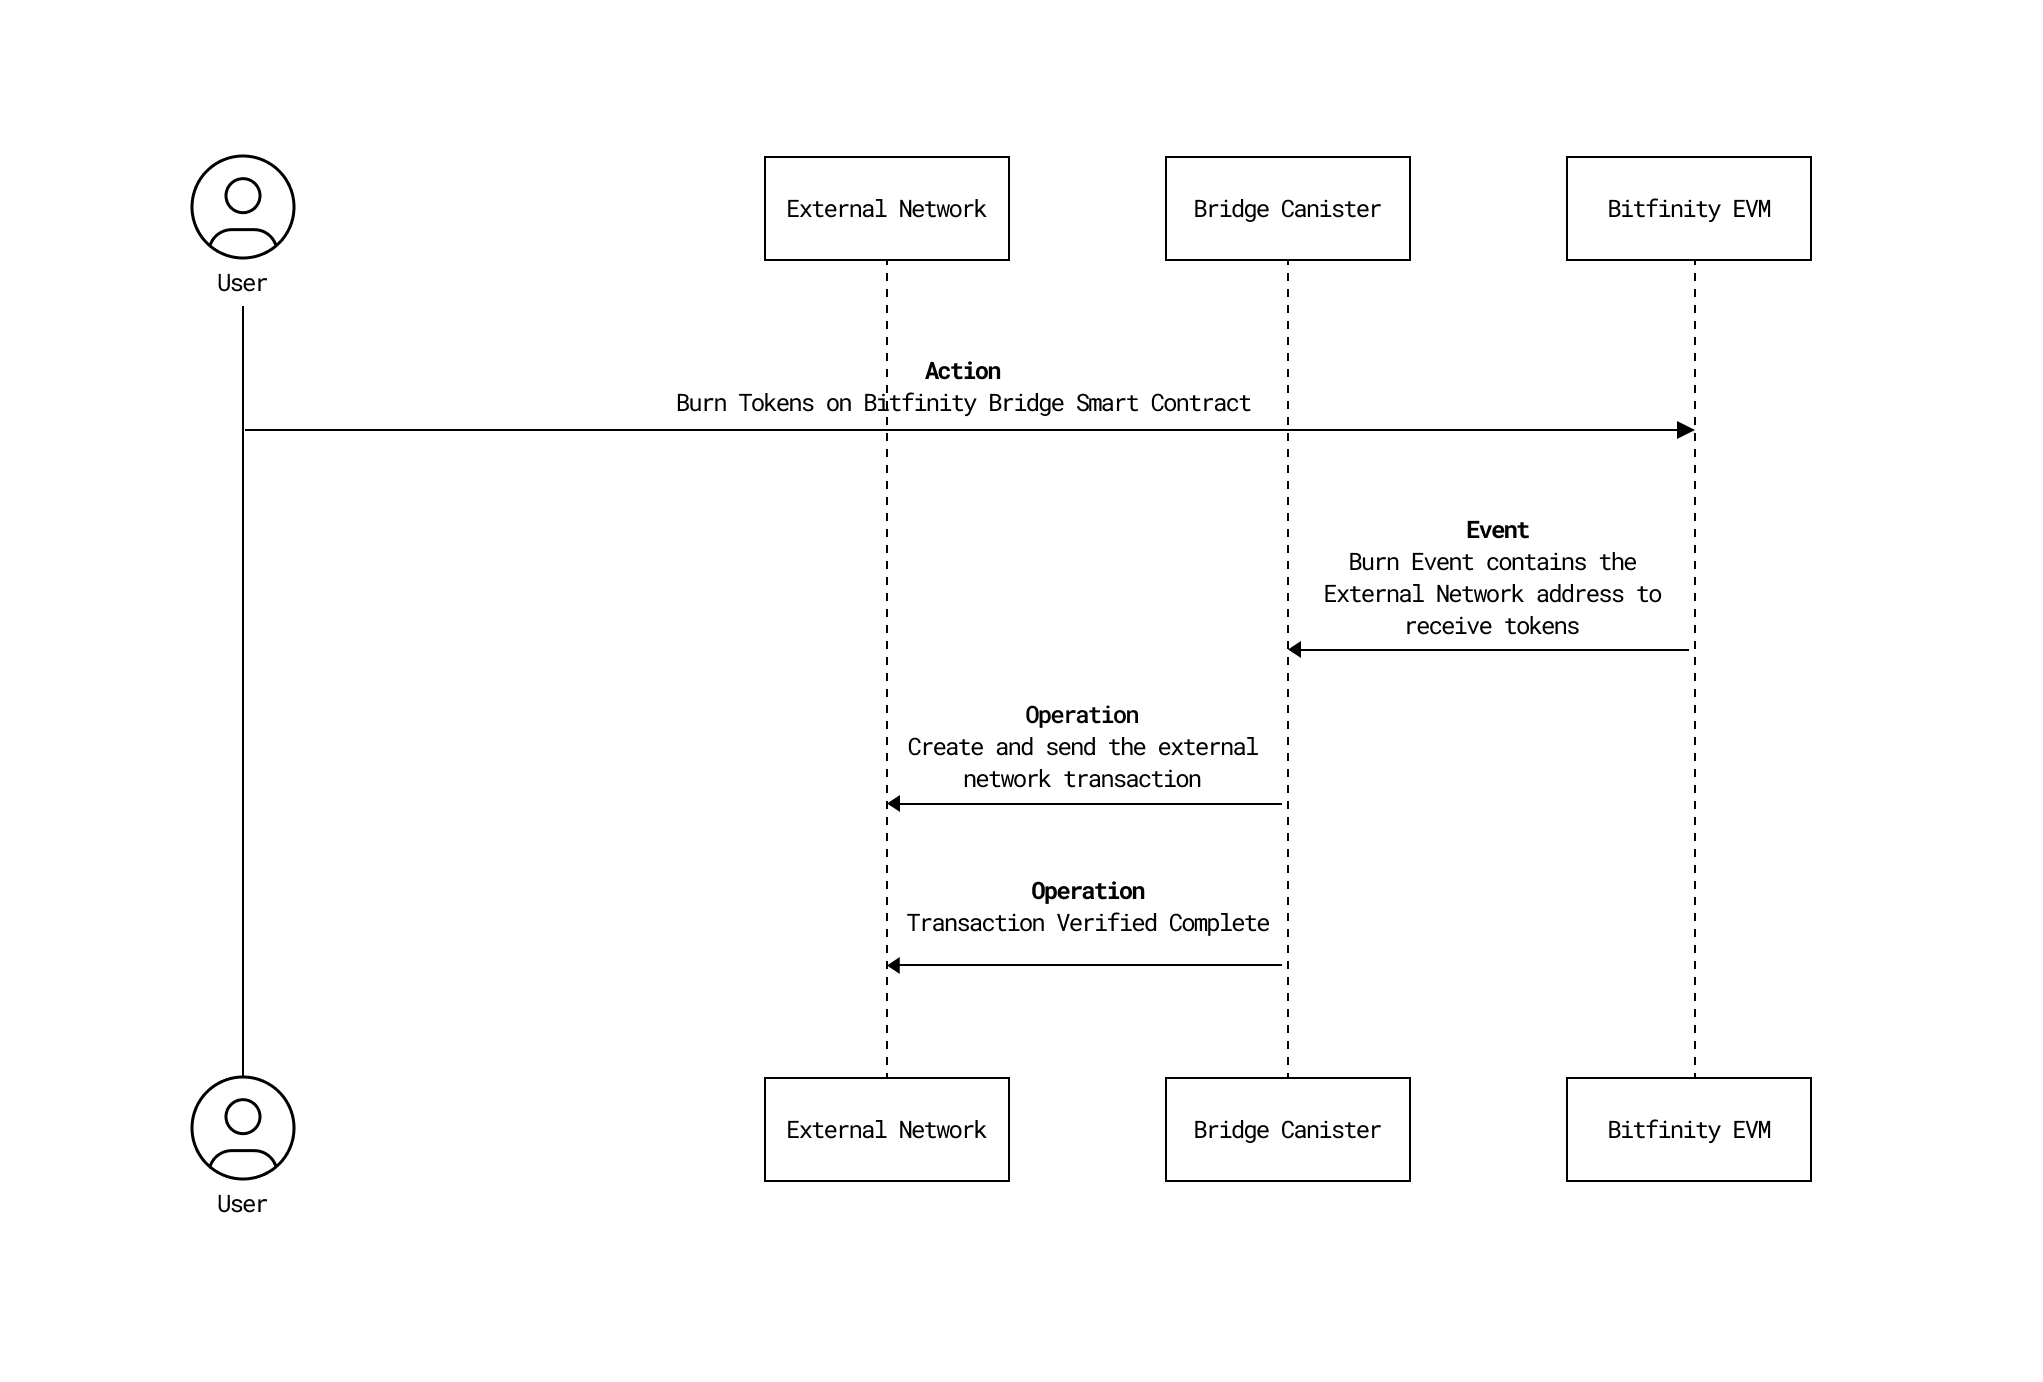
\includegraphics[width=1\textwidth]{standard_withdraw.png}
    \caption{Overview of the standard flow for burning wrapped tokens and withdrawing base chain tokens}
    \label{fig:standard_withdraw}
\end{figure}


The sequence of operations form figure \ref{fig:standard_withdraw} are described below.

    \begin{enumerate}  
        \item{\textbf{WrappedTokenBurned (Event):}} After a user burns wrapped tokens on the bridged chain, the system generates a burn event. The event handler, by default, records this burn information in the canister’s stable storage and schedules a transfer operation accordingly.
        
        \item \textbf{Transfer Base Token (Op)}: The bridge canister issues a transfer of the base chain tokens to the recipient address, parsed from the burn event. 

        \item \textbf{Transaction Verified (Op)}.  This operation verifies the transaction has either completed successfully or failed. In the case of failure, we can revert to the prior stage to enable retries for the transfer.  

 \end{enumerate}

Having detailed the sequence of operations that make up the deposit and withdrawal bridging flows, along with the core components of the BitFusion framework, the subsequent sections will discuss the specific implementation of BitFusion bridges across various blockchain networks, including Bitcoin, Bitcoin Runes, and Ethereum. Our focus will primarily be on the deposit flow for these networks. The withdrawal flow, generally simpler to implement, mainly involves the implementation of signing, sending, and verifying transactions on each respective network.


\section{Bridging Bitcoin}
\subsection{Background on ckBTC}
Canisters can read the state of the Bitcoin blockchain through a network of Bitcoin nodes running on the Internet Computer protocol. Bitcoin that is wrapped here is called Chain-Key Bitcoin (ckBTC), which comprises the following key components:

\begin{itemize}
\item \textbf{Minter Canister:} \texttt{mqygn-kiaaa-aaaar-qaadq-cai}
\item \textbf{Ledger Canister:} \texttt{mxzaz-hqaaa-aaaar-qaada-cai}
\end{itemize}

These canisters interface with the following canisters to query information from the Bitcoin network and also issue threshold signatures:

\begin{itemize}
\item \textbf{Bitcoin Canister:} An OS-level process external to the replica that interacts with Bitcoin nodes through the Bitcoin Adapter. 
\item \textbf{Threshold Signing API:}  through the management canister
\end{itemize}.

The overall architecture for the system can be seen in figure \ref{fig:ckbtc}. The various components are explained in more detail in the section below. 

\begin{figure}[H]
    \centering
    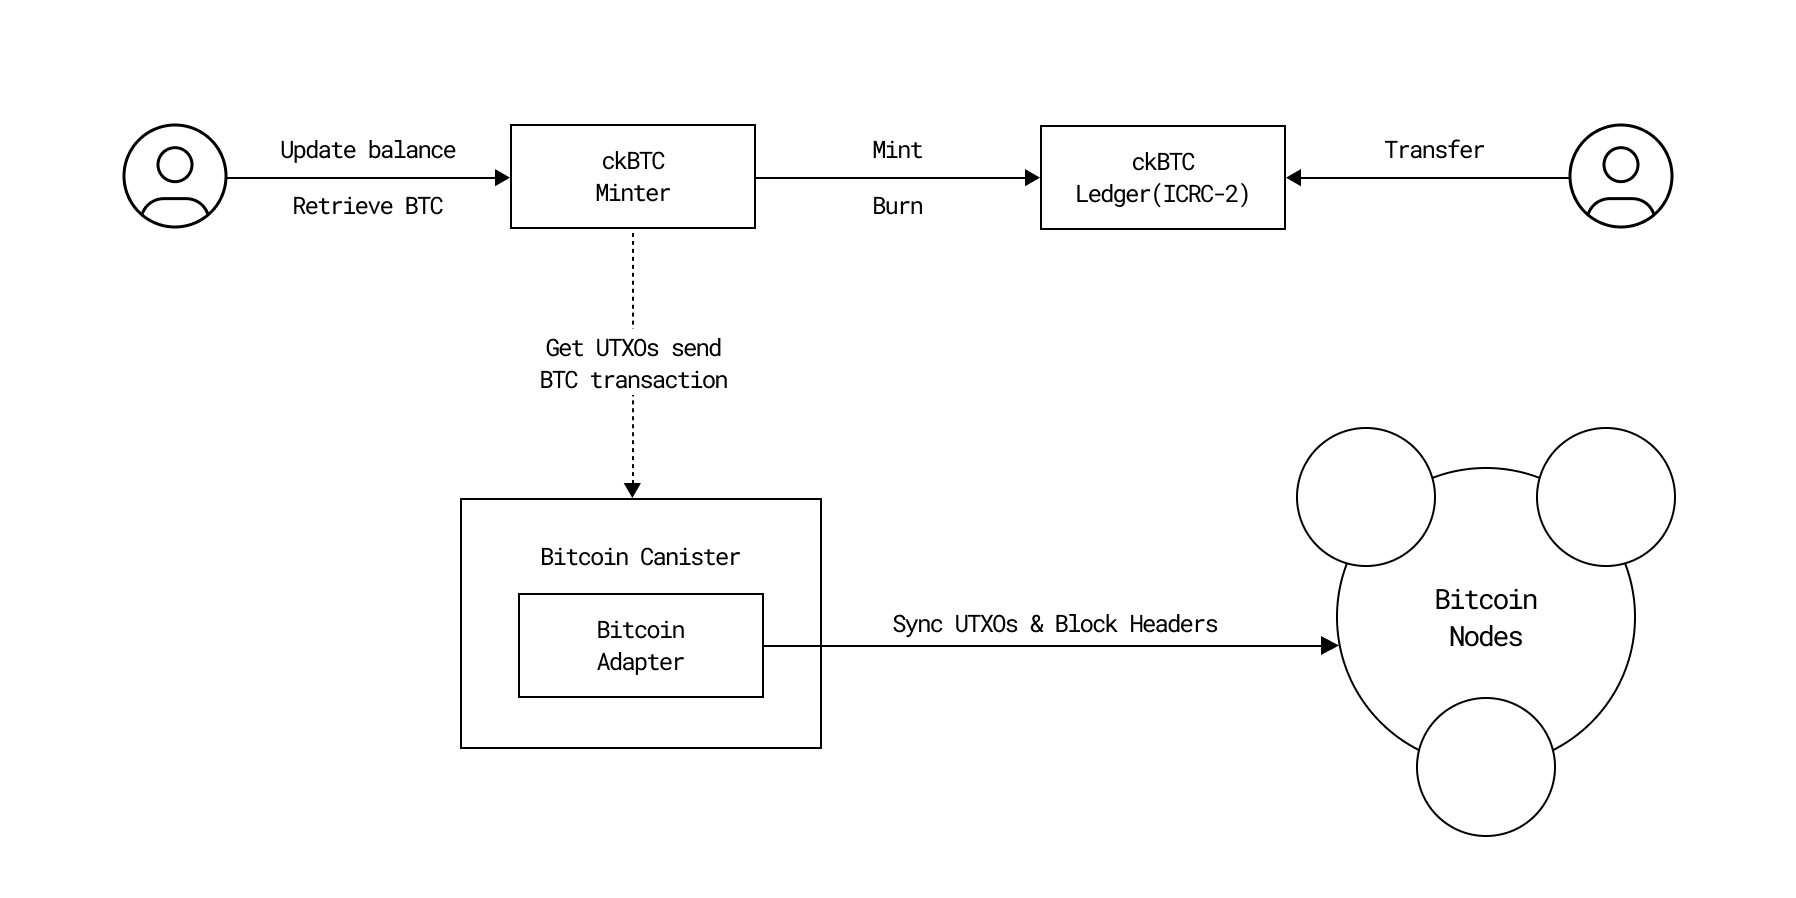
\includegraphics[width=1\textwidth]{ckbtc.png}
    \caption{Overview of the ckBTC architecture and network interface for Bitcoin}
    \label{fig:ckbtc}
\end{figure}

\textbf{ckBTC Minter} The ckBTC Minter Canister interacts with the Bitcoin Canister to query the current Unspent Transaction Output (UTXO) set of the Bitcoin network.  This interaction ensures that the ckBTC Minter Canister can accurately mint ckBTC tokens based on the Bitcoin deposited into an address it controls through the tECDSA API. When the ckBTC Minter Canister issues a Bitcoin transaction, it queries the Bitcoin Canister to retrieve the necessary UTXO information to spend UTXOs and ultimately sign transactions through tECDSA. 

\textbf{Bitcoin Canister}
The Bitcoin Canister is a key component of the integration with the Bitcoin network. It provides the necessary interfaces to interact with Bitcoin, including querying UTXOs, balances, and transaction fees, as well as submitting transactions. The Bitcoin Canister maintains the state by syncing Bitcoin blocks through the Bitcoin Adapter, described in the following paragraph, ensuring that the UTXO set and balances are up-to-date. It handles requests from other canisters to perform Bitcoin operations, like issue transactions or query UTXOs.

The Bitcoin Canister syncs the current UTXO set up to the most recent blockchain header and issues transactions, through the Bitcoin Adapter. This is an OS-level process external to the replica that connects to multiple Bitcoin nodes. It maintains a local copy of the entire block header chain and a small cache of blocks, which it provides to the replica upon request.

For more details, refer to the Bitcoin Integration page \footnote{\href{https://wiki.internetcomputer.org/wiki/Bitcoin_Integration}{Bitcoin integration}}.





\subsection{Bitcoin Deposit Flow}

BitFusion uses ckBTC to facilitate transfers of Bitcoin to the EVM. The deposit process starts with the user sending Bitcoin to the address of their deposit account. This deposit address is an encoding of the user's EVM address as a Bitcoin address, which is controlled through the tECDSA API by the ckBTC minter canister. 

After this action, the user calls the notifyMinter method on the BftBridge contract with the encoded EVM wallet address as an argument. This call will trigger an event that initiates bridging. The sequence of bridge operations can can be seen in figure \ref{fig:bitcoin} . 

    \begin{figure}[h]
        \centering
         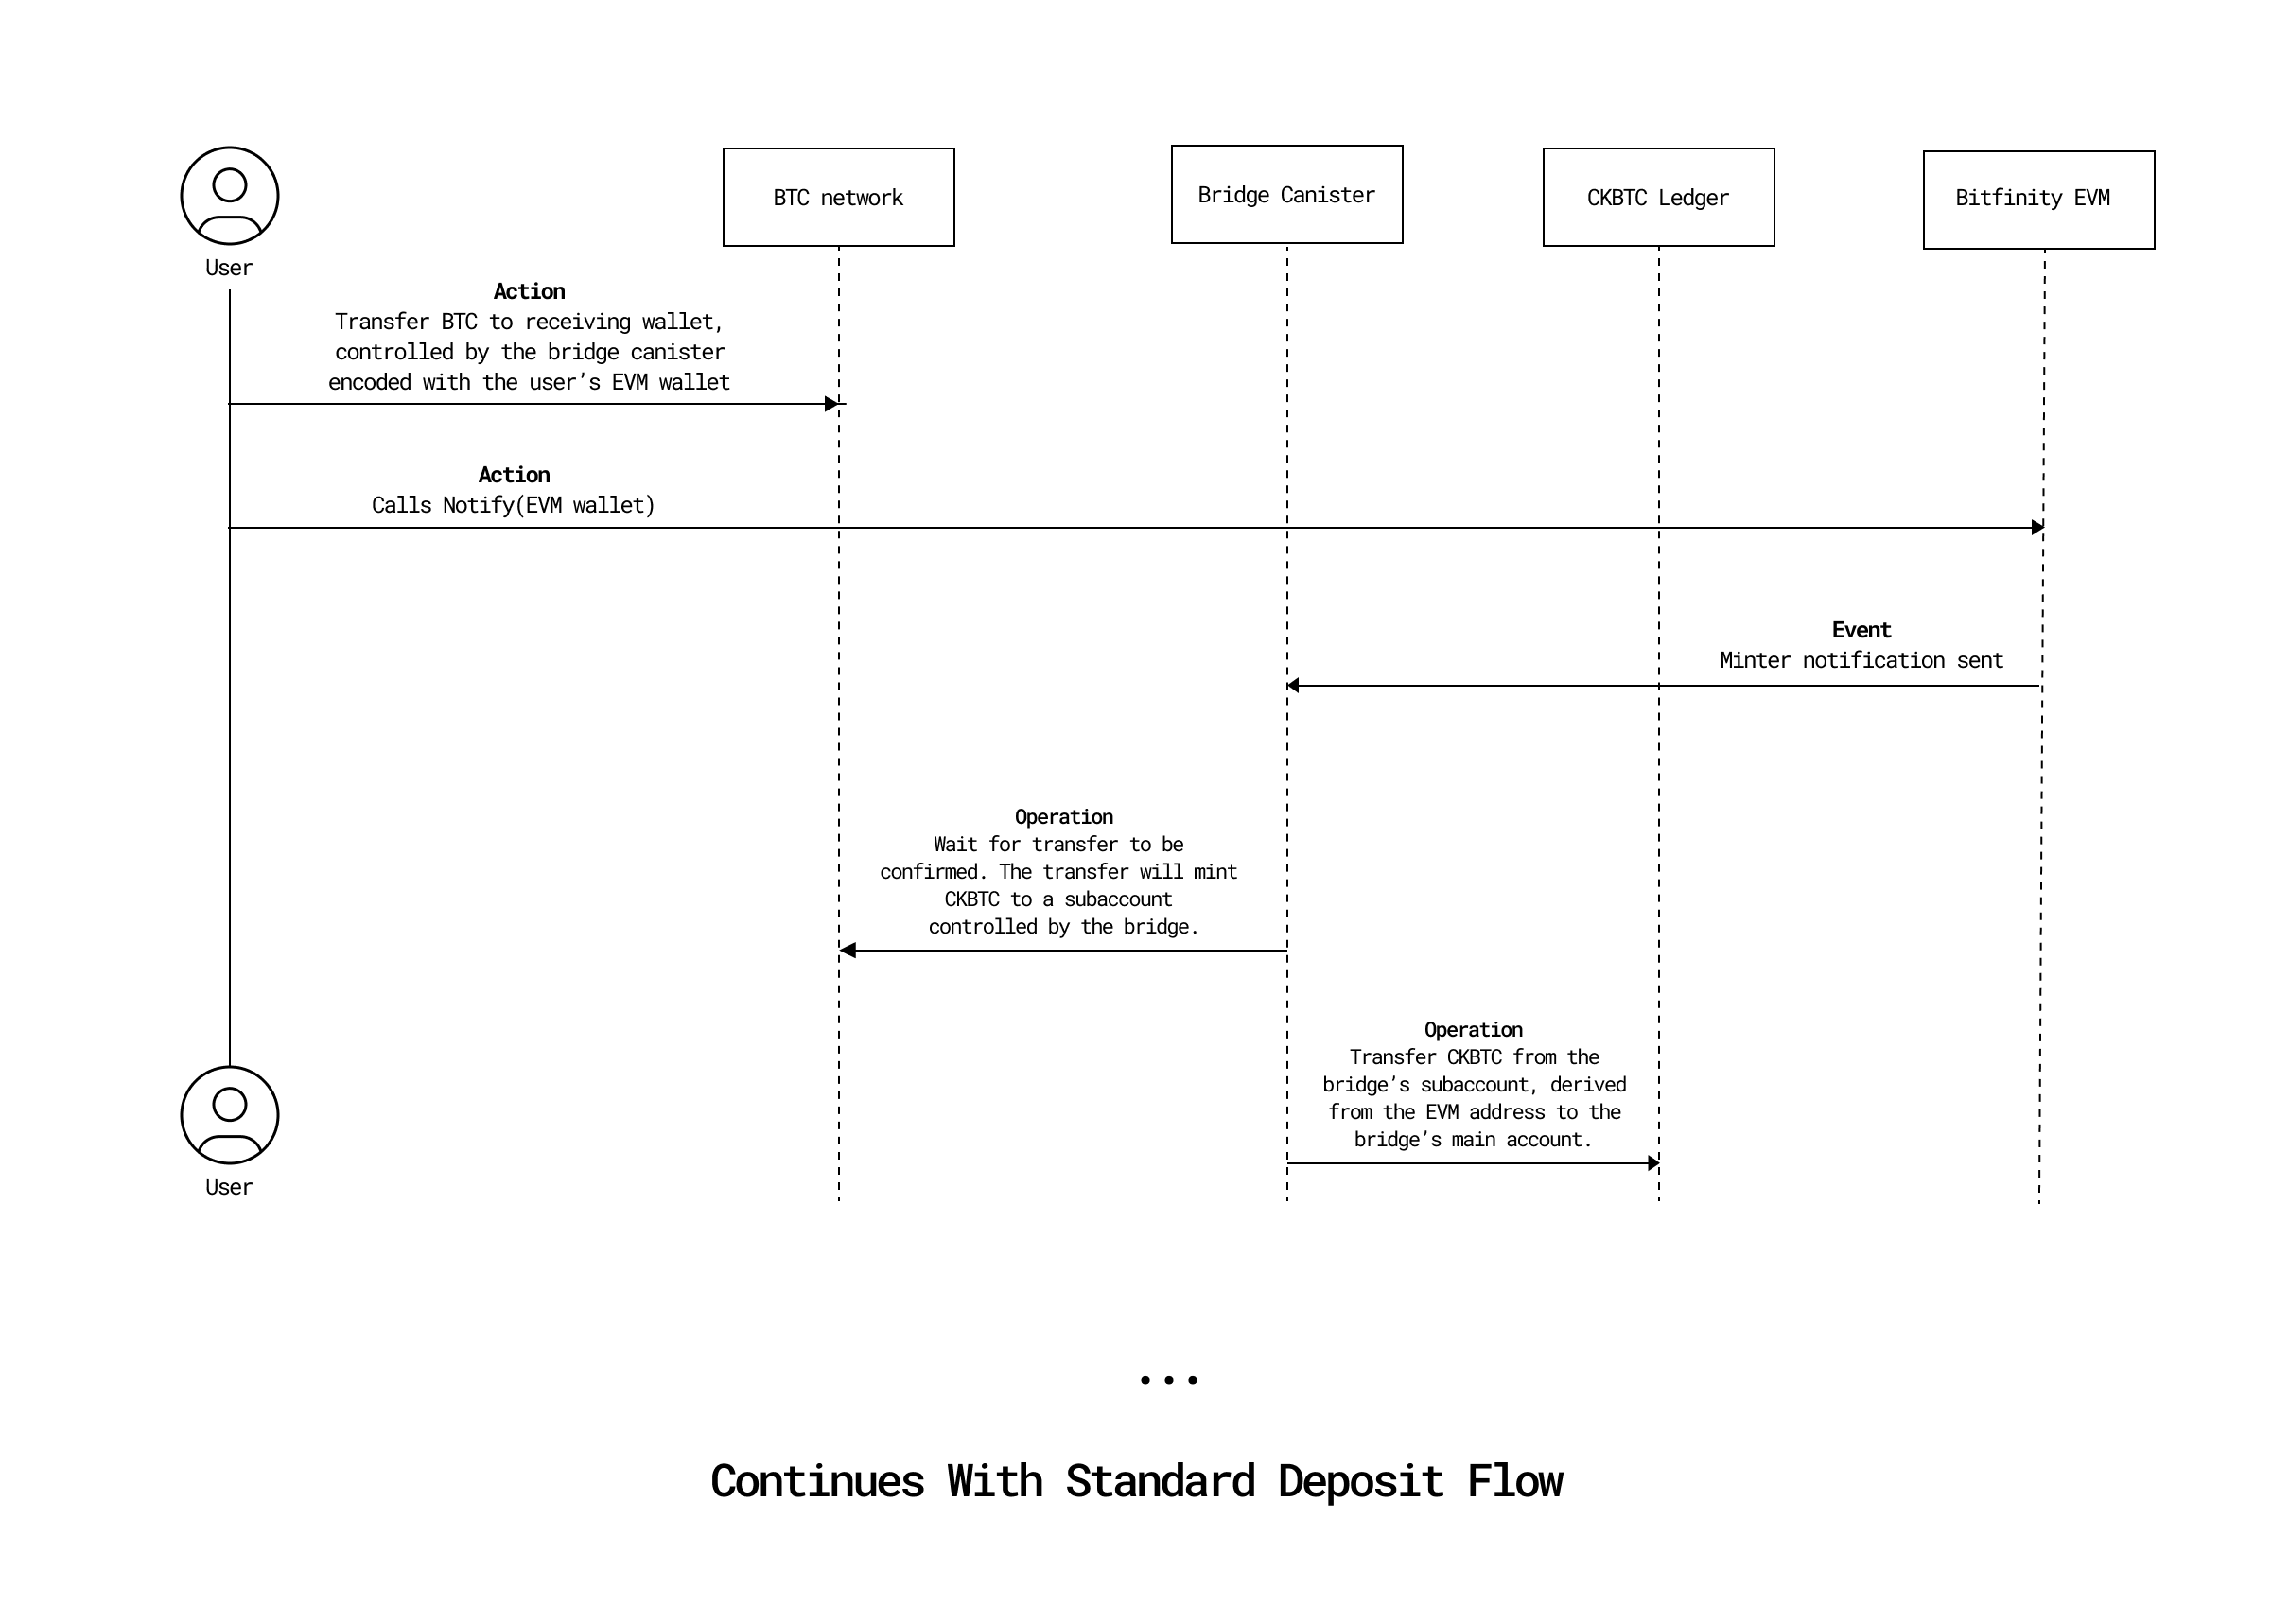
\includegraphics[width=1\textwidth]{bitcoin.png}
        \caption{Overview of ckBTC and the Bitcoin network interface }
        \label{fig:bitcoin}
    \end{figure}

 After the notification event has been processed by the bridge canister, the following sequence of operations will be executed to complete the bridging, as described in the list below: 
 
    \begin{enumerate}  

        \item{\textbf{Mint ckBTC (Operation):}}
         The bridge will periodically poll the Bitcoin Canister until a sufficient number of confirmations are received.  Once this happens, the bridge canister calls the ckBTC minter to mint ckBTC, which will be sent to a ICRC-2 subaccount determined by the user's EVM address but controlled by the bridge canister. 
        
        \item \textbf{Transfer to Main Account (Operation):} After ckBTC tokens are minted, the bridge canister transfers these tokens from the subaccount to its main account and then creates a mint order for wrapped tokens designating the user's EVM address.


        \item \textbf{Continuation of Standard Flow:} From here the standard flow to mint wrapped tokens on the EVM is followed through.

 \end{enumerate}

 \subsection{Bitcoin Withdrawal Flow}
 
 To withdraw Bitcoin from the Bitfinity Network, we follow the template implementation described by \ref{fig:standard_withdraw}. The withdrawal transfer operation is implemented through the bridge canister calling the appropriate method on the ckBTC minter, which exposes an API that burns the ckBTC  and sends the UTXOs to the designated user on the bitcoin network. The tECDSA subnet signs a Bitcoin transaction, on behalf of the ckBTC minter, which is then broadcast to the Bitcoin network through the adapter interface. 


\section{Bridging Runes}

When bridging Runes tokens, the bridge canister communicates directly with the Bitcoin network via the Bitcoin Canister. This is necessary because Runes transactions must include metadata in the \textit{op\_return} flag of a Bitcoin transaction to be valid, requiring the flexibility to sign and send transactions directly.

To index Runes from the Bitcoin network, the bridge canister relies on a separate, configurable Indexer Canister rather than parsing UTXOs on its own. This Indexer Canister can interface with an on-chain Runes indexer, such as the one developed by the \href{https://github.com/octopus-network/ord-canister}{Omnity Protocol}.

Omnity has created a decentralized on-chain indexer for Runes that operates from a canister. This indexer ports the Runes indexing logic from the authoritative Ord library into the canister. The canister accesses Bitcoin block data through the Bitcoin Canister and adapter interface, which provides the header hashes from the Bitcoin blockchain. The indexer processes all Runes block data and serves the information through a canister API, demonstrating the potential for fully decentralized token indexing.

\subsection{Runes Deposit Flow}

To deposit Runes tokens into the bridge, a user must issue a Runes transaction to the designated recipient address. The address is a Bitcoin address controlled by the bridge canister through the tECDSA API that encodes the information on the user's EVM address.

Once the Runes have been sent to this recipient address, a user can invoke the notifyMinter method on the BFTBridge contract to commence the sequence of bridging operations. In figure \ref{fig:runes} below we display the sequence of bridging operations. 


\begin{figure}[H]
    \centering
    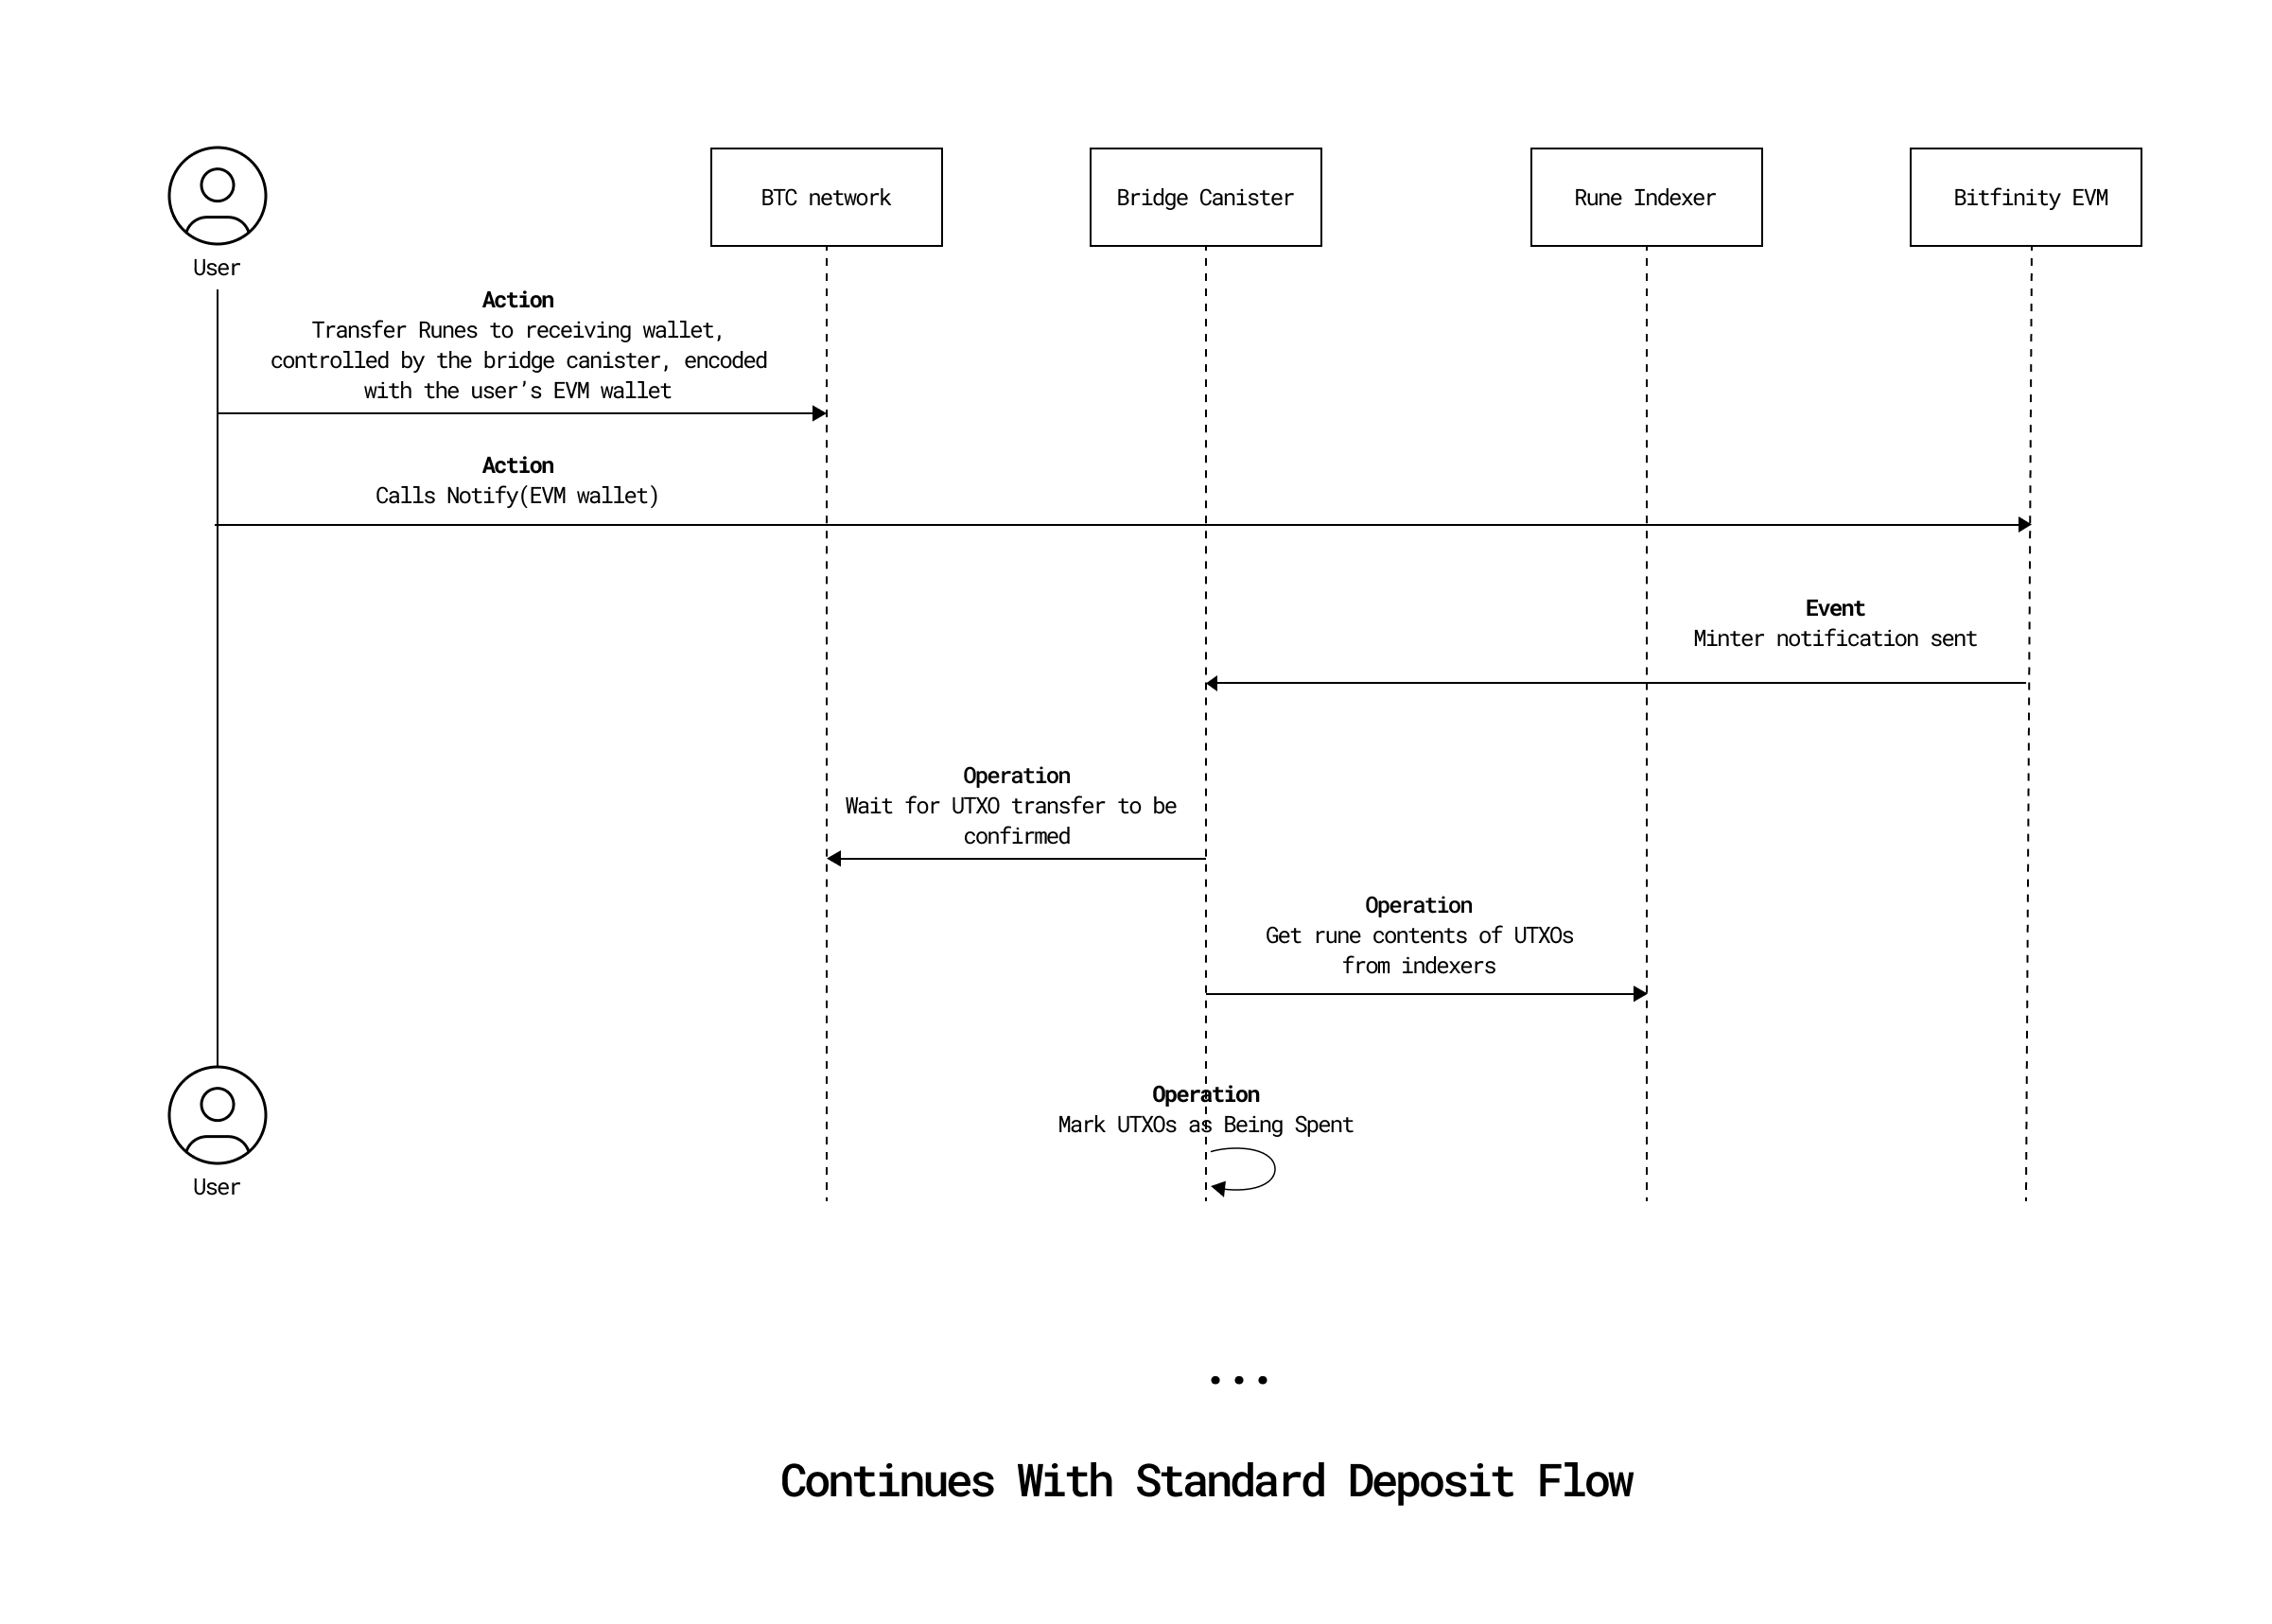
\includegraphics[width=1\textwidth]{runes.png}
    \caption{Overview of the Deposit Flow for Runes tokens}
    \label{fig:runes}
\end{figure}

Upon receiving the event notification and saving the address of the recipient, the bridge canister will undertake the following sequence of operations.

 \begin{enumerate}  
        \item{\textbf{Waits for the UTXO to be Confirmed (Operation):}} The bridge monitors the incoming UTXOs from the Bitcoin network, and waits until they are confirmed by the Bitcoin network.

        \item{\textbf{Retrieve Runes Contents from Indexers (Operation):}} Once the transactions are confirmed, a call is made to the Rune Indexer Canister to retrieve the Runes contents for the transaction.
        
        \item \textbf{Mark UTXOs as Spent (Operation):} After the relevant information has been gathered, the UTXO IDs are marked by the canister as spent/minted to prevent double spending in future Runes deposit requests.

        \item \textbf{Continuation of Standard Flow:} From here the standard flow to mint wrapped tokens on the Bitfinity EVM is followed through.

 \end{enumerate}
 
\subsection{Runes Withdrawal Flow}

The process to withdraw Runes is slightly more involved than for other flows, and a diagram outling the process is show in figure \ref{fig:runes_withdraw}.

\begin{figure}[H]
    \centering
    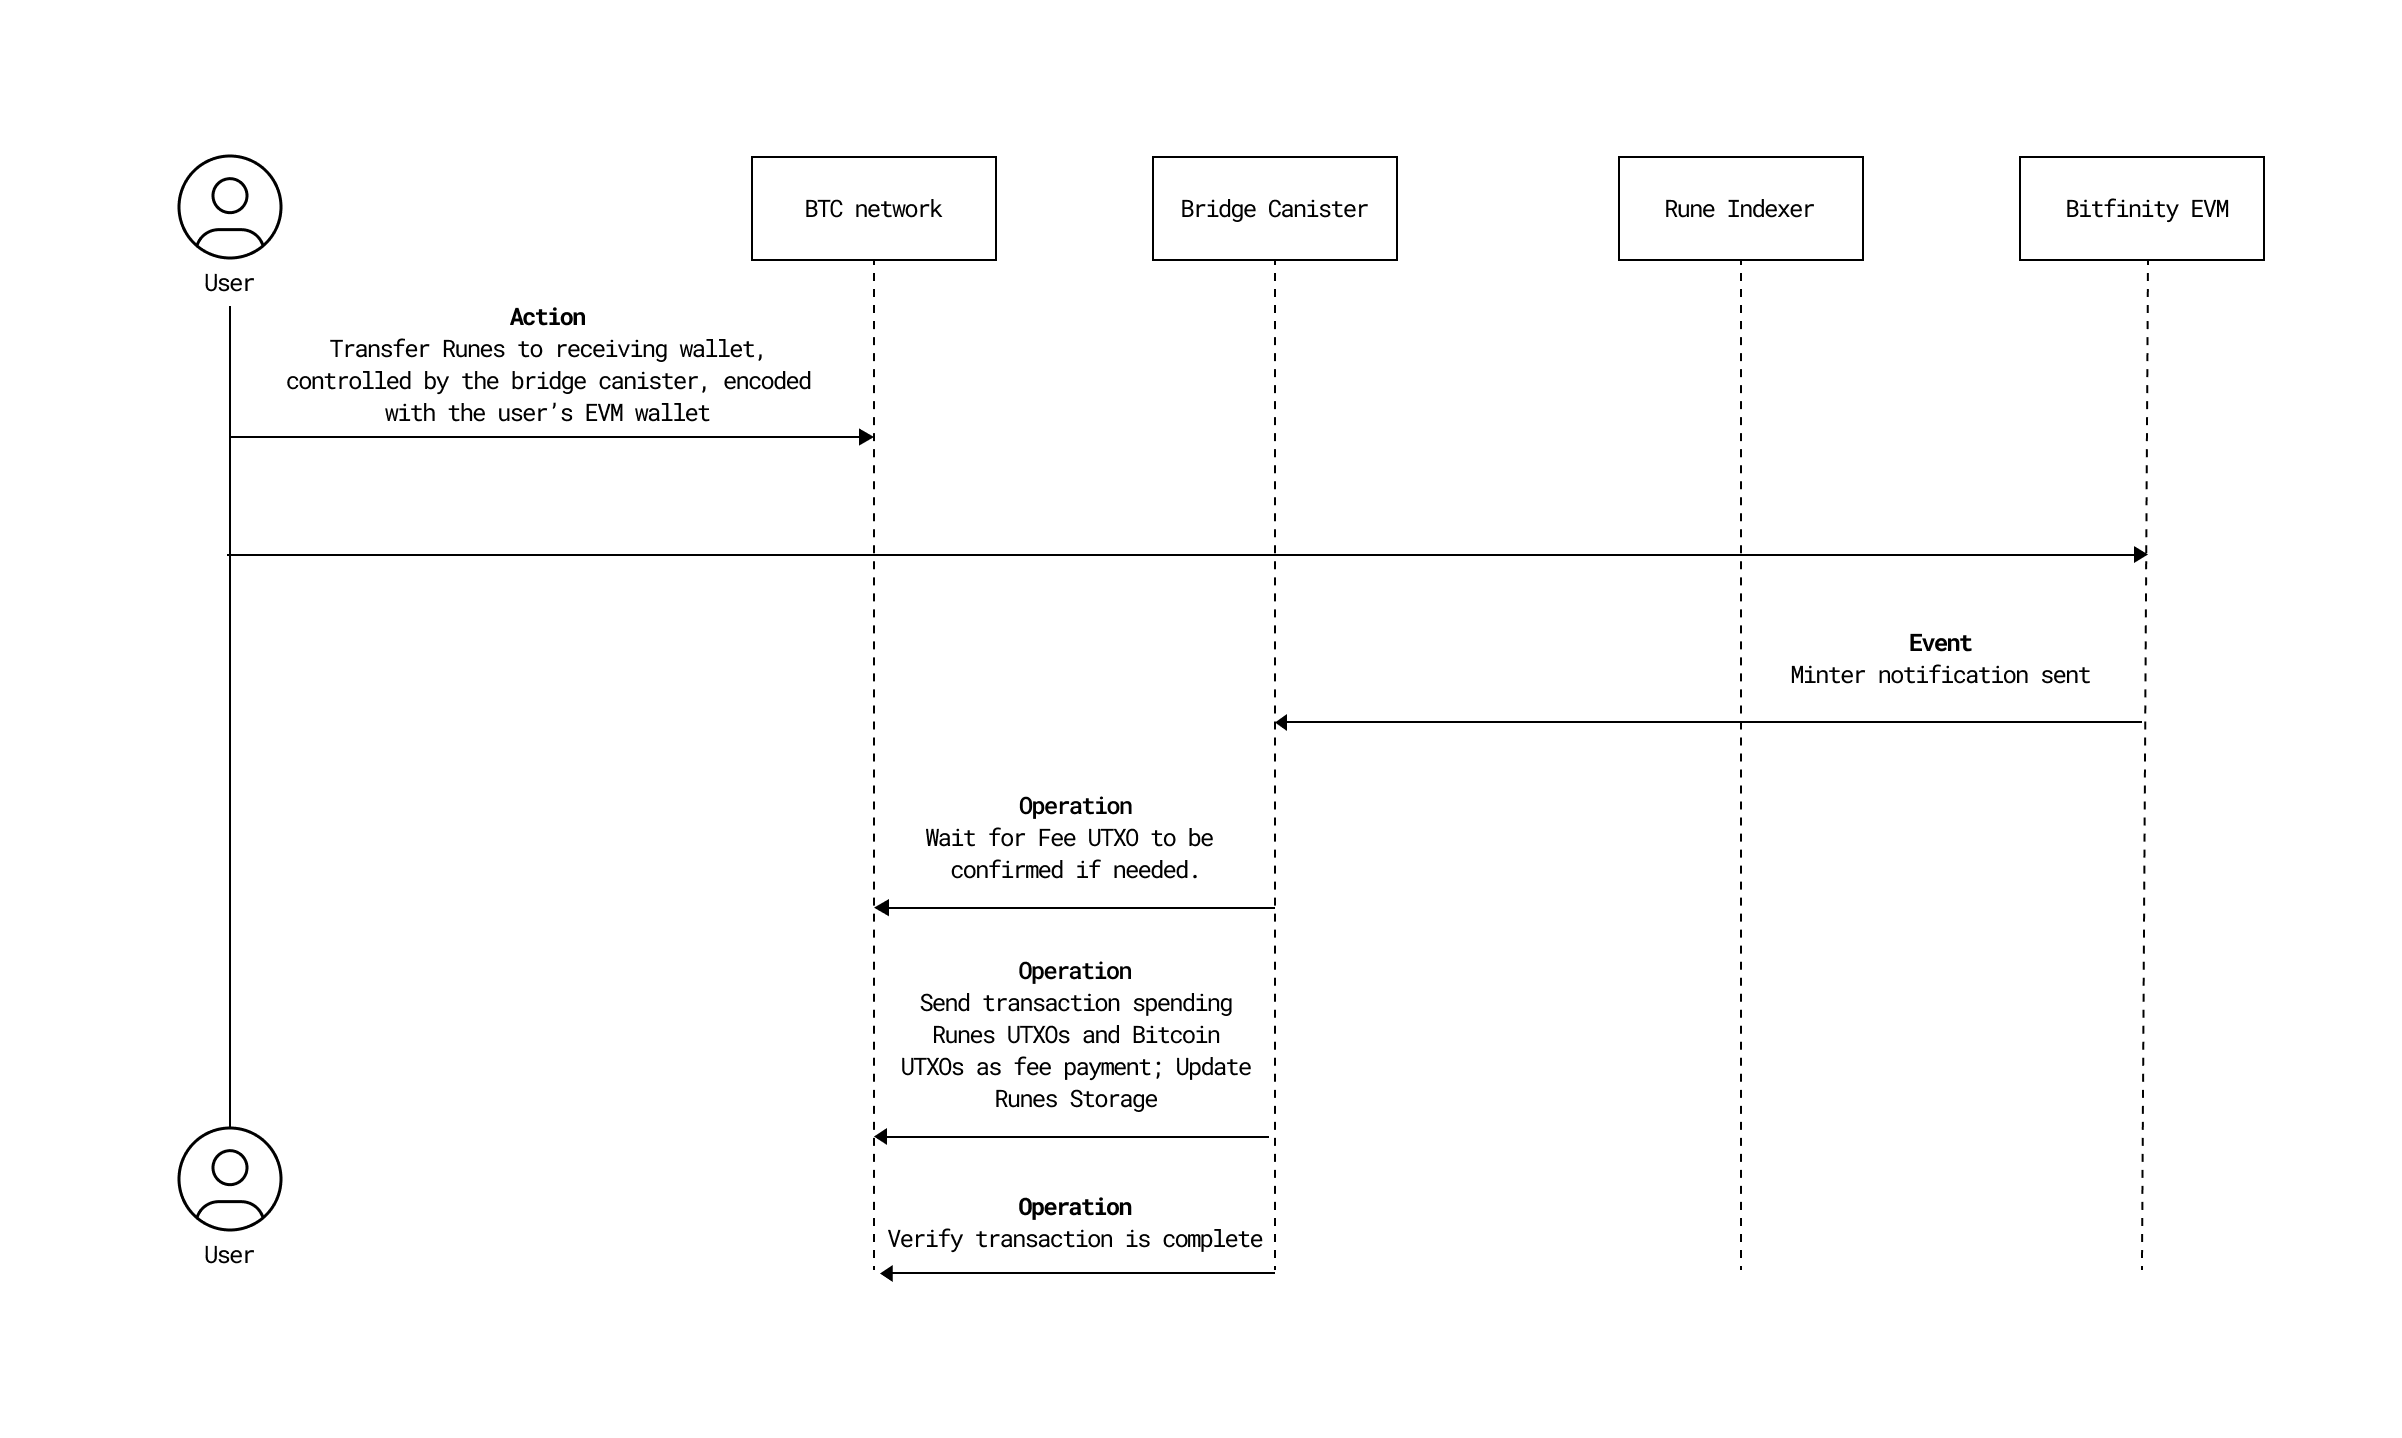
\includegraphics[width=1\textwidth]{runes_withdraw.png}
    \caption{Overview of the Withdrawal Flow for Runes tokens}
    \label{fig:runes_withdraw}
\end{figure}

To withdraw Runes tokens from the bridge, the user must have a sufficient Bitcoin balance on their designated Bitcoin address. To provide fee payment in Bitcoin to facilitate the creation of a withdrawal transaction, the user can send a standard Bitcoin transaction (with no Runes) to the user's designated address. This is the same recipient address as used in Runes bridging. Once the transaction has been mined into a block, it becomes immediately available for the withdrawal process.

After the user initiates the burning of wrapped tokens by calling the burn method on the bridge smart-contract, this will prompt the canister to create a Withdrawal. This transaction utilizes UTXOs containing Runes sufficient to cover the requested withdrawal amount, in addition to those provided as a fee by the user. Any unspent Runes are returned to the main address of the bridge canister, whilst the unspent Bitcoin is sent back to the user's recipient address. 

\section{Bridging ERC-20 Tokens}
\subsection{External EVM Deposit Flow}
Bridging to another EVM chain is relatively straightforward.  To bridge ERC-20 tokens from an external chain, a user must approve the BFTBridge contract deployed to the external chain to spend tokens. Then the user will call the lock method on the smart contract, which will trigger the bridge to lock the tokens in escrow. Once this action has taken place, and the mint notification event is created and received by the bridge canister, bridging proceeds as per the standard flow. See figure \ref{fig:evm} for the deposit flow. 

For the bridge to be fully decentralised, the bridge canister must also have a way of querying the EVM with minimized trust assumptions. One option is to make use of multiple RPC gateways (oracles) to the external EVM chain, ensuring all clients agree before bridging over funds.  For Ethereum in particular, it is possible to query the chain trustlessly through the \href{https://github.com/eigerco/ethereum-canister}{Helios client}, which is an Ethereum light client node implementation that has been implemented as a canister. Helios can verify the proof of stake signatures authenticating block header hashes on Ethereum, and use these header hashes to validate  the entire blockchain. Once the proofs have been obtained, the client can query full nodes and authenticate block data returned against the header hashes it has stored, ensuring its queries are correct. 

\begin{figure}[H]
    \centering
    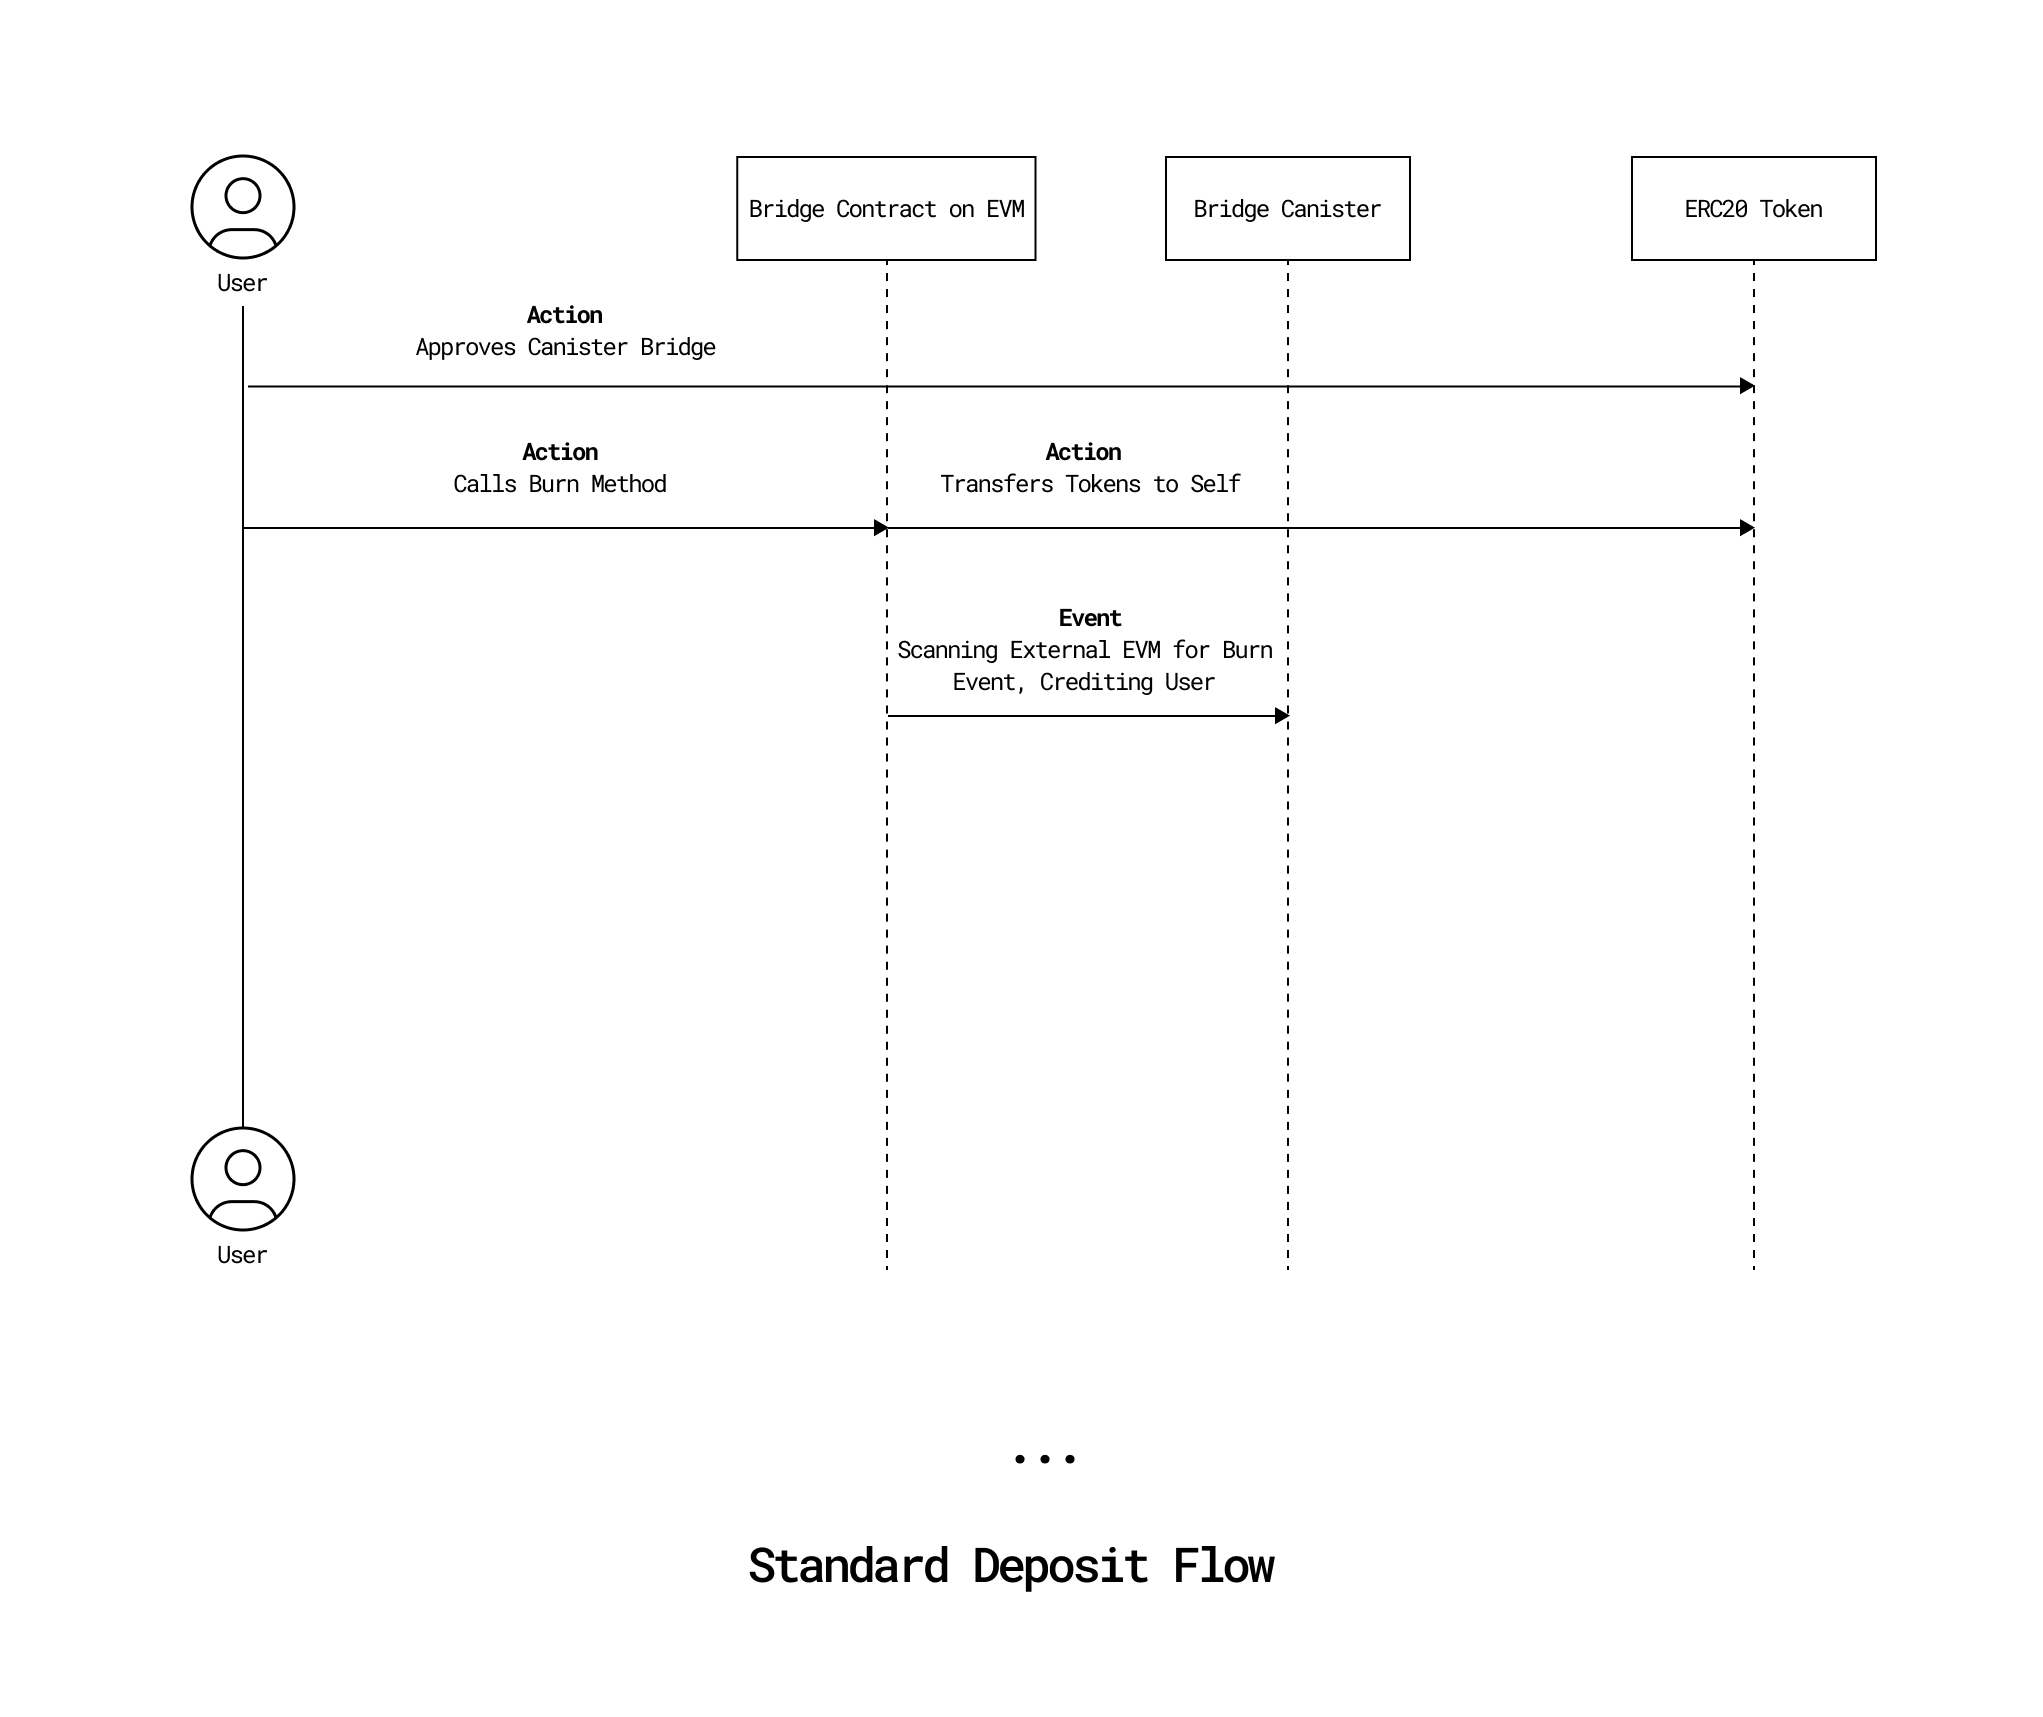
\includegraphics[width=1\textwidth]{evm.png}
    \caption{Overview of the Deposit Flow for EVM tokens}
    \label{fig:evm}
\end{figure}

\subsection{External EVM Withdrawal Flow}

 To withdraw tokens to an EVM network, we follow the template implementation described by the standard withdrawal flow in figure \ref{fig:standard_withdraw}. The withdrawal transfer operation is implemented by issuing an ERC-20 transfer of tokens and broadcasting this transaction to the designated EVM chain. This transaction can then be verified either through the Helios Client running on the network for Ethereum, or by querying oracles for other EVM chains. 


\section{Chain Abstraction}

With the core primitives and security of the bridging flows detailed, we now focus on enhancing the user experience by achieving near-instant bridging between chains.

To accomplish this on BitFusion, an additional layer of abstractions - known as Chain-Abstraction - are necessary. A component of this, Account-Abstraction, introduces a higher-layer construct known as a UserOperation, which acts as a pseudo-transaction object. Users submit these UserOperation objects to a distinct mempool, where ``bundlers'' aggregate them into a single transaction via a special contract. This bundled transaction is then included in a block. Account abstraction shifts the paradigm from externally owned accounts (EOAs) to smart contract wallets that incorporate arbitrary verification logic, enhancing wallet designs and simplifying cross-chain interactions for end-users.

On Bitcoin, a smart wallet could initiate a bridging transaction via a ``Relay Pool." In this setup, relayers with pre-bridged tokens on the destination chain deliver the bridged assets to the user in exchange for a liquidity fee, later receiving the user’s bridged assets from the smart wallet, with the smart wallet being orchestrated by a smart-contract or canister using Chain-Key, for instance. This mechanism facilitates nearly instantaneous cross-chain transfers without waiting for finality on the originating chain. For further details, refer to \cite{uma}.

As a bridge framework, BitFusion enables relayers to use its protocol to transfer their assets, ensuring compatibility with the proposed solution for instantaneous cross-chain liquidity. The introduction of Chain Abstraction and smart wallets has the potential to significantly enhance the bridging experience, and these innovations can be seamlessly integrated within BitFusion's adaptable framework.

\section{Comparative Analysis of Bitcoin Layer-2s}

With the core primitives, security, and potential enhancements to user experience through Chain Abstraction detailed, we now shift our focus to a comparative analysis. This section will compare Bitfinity's bridging solution to those used by other Bitcoin Layer-2 solutions, emphasizing their capabilities in terms of security, decentralization, and integration with the Bitcoin network.

The following tables highlight key features of Bitfinity, Merlin, RSK, STACKS, and BOB protocols. Specifically, the analysis covers the size of the membership for the MPC signing group holding Bitcoin, whether the MPC committee has adaptive membership, the ability of the committee to re-share and delete stale keys, the validation of Bitcoin block headers through consensus, merge mining support with Bitcoin, and the degree to which the bridging framework is modular and extensible to new tokens in the Bitcoin ecosystem.


\vspace{1cm}


\begin{table}[H]
    \centering
    \renewcommand{\arraystretch}{1.5} % Increase the row height
    \begin{tabular}{|l|c|c|c|c|c|}
        \hline
        \textbf{Feature} & \textbf{Bitfinity} & \textbf{Merlin} & \textbf{RSK} & \textbf{STACKS} & \textbf{BOB} \\
        \hline
        \textbf{Group Size} & 28+ & ? & 5-of-9 & 3rd party bridge & 3-of-5 \\
        \hline
        \textbf{Adaptive Membership} & Yes & No & No & No & No \\
        \hline
        \textbf{Keys Re-shared} & Yes (every 10 mins) & No & No & No & No \\
        \hline
        \textbf{BTC Blocks Validated} & Yes & No & Yes & Yes & Yes \\
        \hline
        \textbf{On-Chain Indexers} & Yes & No & No & No & No \\
        \hline
        \textbf{Merge Mining} & No & No & Yes & Yes & Yes \\
        \hline
        \textbf{Modular Bridging} & Yes & No & No & No & No \\
        \hline
    \end{tabular}
    \caption{Comparative Analysis of Bitcoin Layer-2 Protocols}
    \label{tab:comparative_analysis}
\end{table}


Bitfinity performs favorably in several key areas, making it a strong choice for developers and users within the Bitcoin Layer-2 ecosystem. The security of its signature scheme is robust, featuring adaptive membership that allows participants to join and leave dynamically, with stale key shares being deleted. Additionally, Bitfinity supports on-chain indexers for tokens in the Bitcoin ecosystem, and the modular bridging setup facilitates extensions to new token types. These features collectively position Bitfinity as a strong option for developers who value security and flexibility.  


\section{Conclusion}

The BitFusion framework significantly enhances the Bitcoin ecosystem, facilitating closer integration with EVM networks through secure and decentralized bridging methods. Utilizing Chain-Key cryptography, a robust threshold Elliptic Curve Digital Signature Algorithm (tECDSA), and directly interfacing with a network of nodes on the Bitcoin network, BitFusion maintains the high-security standards essential for Bitcoin developers and closes the gap between the security of bridging solutions and proof-of-stake blockchains.

BitFusion’s use of a decentralized Runes indexer, deployed to a canister, in the bridging flow enhances security and reliability when bridging new tokens on the Bitcoin blockchain. This addresses a critical question: how to enable decentralized applications to interact securely with new Bitcoin-based tokens. The framework's modular and scalable architecture provides developers with substantial flexibility to innovate and develop unique bridging applications. This paper presents three such implementations, showcasing the framework's capabilities and setting the stage for further community-driven advancements in the field.





\nocite*{}
\bibliographystyle{alpha}
\bibliography{sample}




\end{document}